\documentclass[12pt,italian]{article}
\usepackage[italian]{babel}
\usepackage[a4paper, margin=1.97cm]{geometry}
\usepackage{graphicx}
\usepackage{amsmath}
\usepackage{subcaption}
\usepackage[dvipsnames]{xcolor}
\usepackage[
    colorlinks=true,
    linkcolor=blue,
    citecolor=blue,
    urlcolor=blue
]{hyperref}
\usepackage{cleveref}
\usepackage{csquotes}
\usepackage[style=phys, backend=biber, biblabel=brackets]{biblatex}

\graphicspath{{./images/}}
\addbibresource{bibliografia.bib}

\DeclareFieldFormat{postnote}{\textcolor{blue}{\mkpageprefix[pagination]{#1}}}
\DeclareFieldFormat{multipostnote}{\textcolor{blue}
{\mkpageprefix[pagination]{#1}}}
\DeclareFieldFormat{cite}{\hyperref{\mkbibbrackets{#1}}}

\crefformat{equation}{#2(#1)#3}
\crefformat{appendix}{#2(#1)#3}
\crefname{table}{tab.}{tab.}

\renewcommand{\mkbibbrackets}[1]{\textcolor{blue}{[#1]}}
\newcommand{\err}[1]{\textcolor{red}{#1}}
\newcommand{\ext}[1]{\textcolor{blue}{#1}}


\title{Percolazione e robustezza nelle reti complesse: analisi della transizione di fase nel modello Erdős-Rényi-Gilbert}
\author{Giacomo Cicala}
\date{\today}

\begin{document}
\maketitle

\renewcommand{\abstractname}{Abstract}

\section{Introduzione}
Negli ultimi decenni, lo studio dei sistemi complessi ha subito una profonda accelerazione grazie allo sviluppo della \emph{Network Science}, un framework teorico che permette di descrivere sistemi apparentemente disparati, dalle reti metaboliche nella cellula, alle infrastrutture tecnologiche come Internet, fino alle reti sociali, attraverso un linguaggio matematico unificato.
Una delle questioni centrali in questo ambito riguarda l'emergere spontaneo di proprietà macroscopiche a partire da interazioni locali disordinate. In particolare, è fondamentale comprendere i meccanismi che garantiscono la connettività globale del sistema e, di riflesso, la sua \emph{robustezza} a fronte di fallimenti casuali dei componenti (\emph{random failures}).

Il presente elaborato si propone di analizzare la stabilità strutturale delle reti attraverso lo studio della \emph{teoria della percolazione}, applicata al modello di grafi casuali di Erdős-Rényi $G(N, p)$.
Come discusso da Newman \cite{newman2018networks}, la percolazione rappresenta una delle transizioni di fase geometriche più semplici e fondamentali: essa descrive il passaggio improvviso da uno stato frammentato, in cui il sistema è composto da isole disconnesse, a uno stato connesso dominato da una \emph{componente gigante} che connette l'intero sistema.

Sebbene le reti reali presentino spesso correlazioni complesse, il modello di Erdős-Rényi-Gilbert costituisce il "modello nullo" di riferimento, analogo al gas ideale in termodinamica.

\subsection{Obiettivi del lavoro}
Lo scopo centrale di questo elaborato è lo studio della \emph{teoria della percolazione} come chiave di lettura per comprendere le transizioni di fase e la resilienza nelle reti complesse.
Utilizzando il modello di Erdős-Rényi-Gilbert come sistema di riferimento analitico, il lavoro si prefigge i seguenti obiettivi:

\begin{itemize}
    \item \textbf{Analisi teorica e computazionale dei fenomeni critici:} Studio della transizione di fase continua che porta all'emersione dell'ordine macroscopico (la \emph{componente gigante}). Dal punto di vista analitico, si ricaverà la soglia critica $\langle k \rangle_c = 1$ e si studierà il comportamento asintotico del parametro d'ordine $S$ e della suscettività topologica $\chi$. Computazionalmente, si verificheranno le leggi di \emph{scaling} universali tramite simulazioni numeriche su \emph{ensemble} di grafi, estraendo gli esponenti critici $\beta$ e $\gamma$ mediante \emph{fit}.

    \item \textbf{Percolazione inversa e robustezza:} Valutazione teorica e numerica della stabilità del \emph{network} a fronte di fallimenti casuali (\emph{random failures}). Teoricamente, si ricaverà la frazione critica di nodi rimossi $f_c = 1 - 1/\langle k \rangle$ necessaria per causare il collasso funzionale del sistema. Questo processo verrà riprodotto computazionalmente, allo scopo di estrarre empiricamente le soglie di percolazione al variare della connettività iniziale e verificare tramite fit la validità della legge teorica.
\end{itemize}
\section{Elementi di teoria dei grafi}
Prima di addentrarci nell'analisi del modello di Erdős-Rényi-Gilbert, è necessario introdurre alcuni concetti fondamentali della teoria dei grafi \cite{barabasi2016network}. Un grafo $G$ è costituito da un insieme di nodi e un insieme di link che connettono coppie di nodi, rappresentando un'interazione tra di essi. La dimensione del grafo è data dal numero di nodi $N$, mentre la connettività è data dal numero totale di link $L$.
Una proprietà fondamentale di ciascun nodo è il suo grado $k$, che rappresenta il numero di link che esso possiede verso altri nodi.
In un grafo non orientato, il numero totale di link $L$, può essere espresso come:
\begin{equation}
    L = \frac{1}{2} \sum_{i=1}^{N} k_i
\end{equation}
dove $k_i$ è il grado del nodo $i$. Il grado medio $\langle k \rangle$ è dato da:
\begin{equation}
    \langle k \rangle = \frac{1}{N} \sum_{i=1}^{N} k_i = \frac{2L}{N}
    \label{eq:grado_medio}
\end{equation}
La distribuzione dei gradi, $P(k)$, fornisce la probabilità che un nodo scelto casualmente nella rete abbia grado $k$. Poiché $P(k)$ è una probabilità, deve essere normalizzata, cioè:
\begin{equation}
    \sum_{k=1}^{\infty} P(k) = 1
\end{equation}
Per una rete con $N$ nodi, la distribuzione dei gradi è data da:
\begin{equation}
    P(k) = \frac{N_k}{N}
\end{equation}
dove $N_k$ è il numero di nodi di grado $k$.
\section{Modello di Erdős-Rényi-Gilbert}
Il modello di Erdős-Rényi-Gilbert \cite{newman2018networks}, denotato come $G(N, p)$, è un modello di grafo casuale in cui ogni coppia di $N$ nodi è connessa da un link con probabilità $p$.
In questo modello, il numero totale di link $L$ è una variabile casuale che segue una distribuzione binomiale
\begin{equation}
    P(L) = \binom{\binom{N}{2}}{L} p^L (1-p)^{\binom{N}{2} - L}
\end{equation}
con media
\begin{equation}
    \langle L \rangle = p \binom{N}{2}
\end{equation}
Di conseguenza, utilizzando \cref{eq:grado_medio} il grado medio $\langle k \rangle$ è dato da
\begin{equation}
    \langle k \rangle = \frac{2 \langle L \rangle}{N} = p (N - 1)
\end{equation}
Anche la distribuzione dei gradi $P(k)$ risulta essere binomiale:
\begin{equation}
    P(k) = \binom{N-1}{k} p^k (1-p)^{N-1-k}
\end{equation}
In molti casi siamo interessati a grandi network con grado medio finito $\langle k \rangle$ indipendente dalla dimensione $N$. In questo limite, ovvero $ \langle k \rangle \ll N $, la distribuzione dei gradi tende alla distribuzione di Poisson:
\begin{equation}
    P(k) = \frac{\langle k \rangle^k e^{-\langle k \rangle}}{k!}
\end{equation}

\section{Transizione di fase di percolazione}
\subsection{Emergenza della componente gigante}
Consideriamo il caso in cui $p = 0$: non vi sono link nella rete ed essa è completamente sconnessa. Nel limite opposto, quando $p = 1$, ogni vertice è connesso direttamente a tutti gli altri, creando un'unica componente che copre l'intera rete. Concentriamoci ora sulla dimensione della componente più grande della rete in ciascuno di questi casi: nel primo caso ($p = 0$) la componente più grande ha dimensione 1, el secondo ($p = 1$) la componente più grande ha dimensione $N$ (ovvero è estensiva). \ext{ In molte applicazioni delle reti è cruciale che esista una componente che riempia la gran parte della rete. Per esempio, nel caso di Internet, è importante che vi sia un cammino attraverso la rete che colleghi la maggior parte dei computer alla maggior parte degli altri. Se così non fosse, la rete non sarebbe in grado di svolgere la sua funzione prevista di garantire le comunicazioni computer-computer per i suoi utenti}.

Una domanda interessante da porsi è come avvenga la transizione tra questi due estremi se costruiamo grafi casuali con valori di $p$ gradualmente crescenti, partendo da 0 e finendo a 1. Potremmo intuire, per esempio, che la dimensione della componente più grande aumenti in qualche modo gradualmente con $p$, diventando estensiva solo nel limite in cui $p = 1$. In realtà, la dimensione della componente più grande subisce un cambiamento improvviso, o transizione di fase, da dimensione costante a dimensione estensiva in corrispondenza di un particolare valore speciale di $p$. Una componente della rete la cui dimensione cresce proporzionalmente a $N$ è chiamata componente gigante. La dimensione della componente gigante $S$, definita come la frazione di nodi che vi appartengono, nel limite di Poisson è data dall'equazione trascendente:
\begin{equation}
    S = 1 - e^{-\langle k \rangle S}
    \label{eq:giant_comp}
\end{equation}
e il punto critico di percolazione, ovvero il punto in cui la componente gigante emerge, è dato da
\begin{equation}
    \langle k \rangle_c = 1
\end{equation}
come ricavato in \cref{sec:GC}.

Possiamo distinguere quattro regimi topologici distinti \cite{barabasi2016network} \cref{fig:regimes} in funzione del grado medio $\langle k \rangle$:
\begin{enumerate}
    \renewcommand{\labelenumi}{\alph{enumi}.}
    \item \textbf{Regime subcritico ($\langle k \rangle < 1$):} In questo regime, la rete è composta da numerosi cluster finiti di dimensione limitata. La dimensione massima dei cluster cresce al massimo come $\log N$, e non esiste una componente gigante. La rete è frammentata e non connessa.

    \item \textbf{Punto critico ($\langle k \rangle = 1$):} In questo punto, la rete subisce una transizione di fase. La dimensione massima dei cluster cresce come $N^{2/3}$, e la suscettività topologica diverge. La rete è ancora frammentata, ma si avvicina alla formazione di una componente gigante.

    \item \textbf{Regime supercritico ($\langle k \rangle > 1$):} In questo regime, emerge una componente gigante che contiene una frazione finita $S$ dei nodi. I cluster finiti rimanenti hanno dimensione limitata. La rete è connessa a livello macroscopico.

    \item \textbf{Regime completamente connesso ($\langle k \rangle > \ln N$):} In questo regime, il numero di aspettazione di nodi isolati è inferiore a 1, e la rete è quasi sicuramente completamente connessa.
\end{enumerate}

\begin{figure}[htbp]
    \centering
    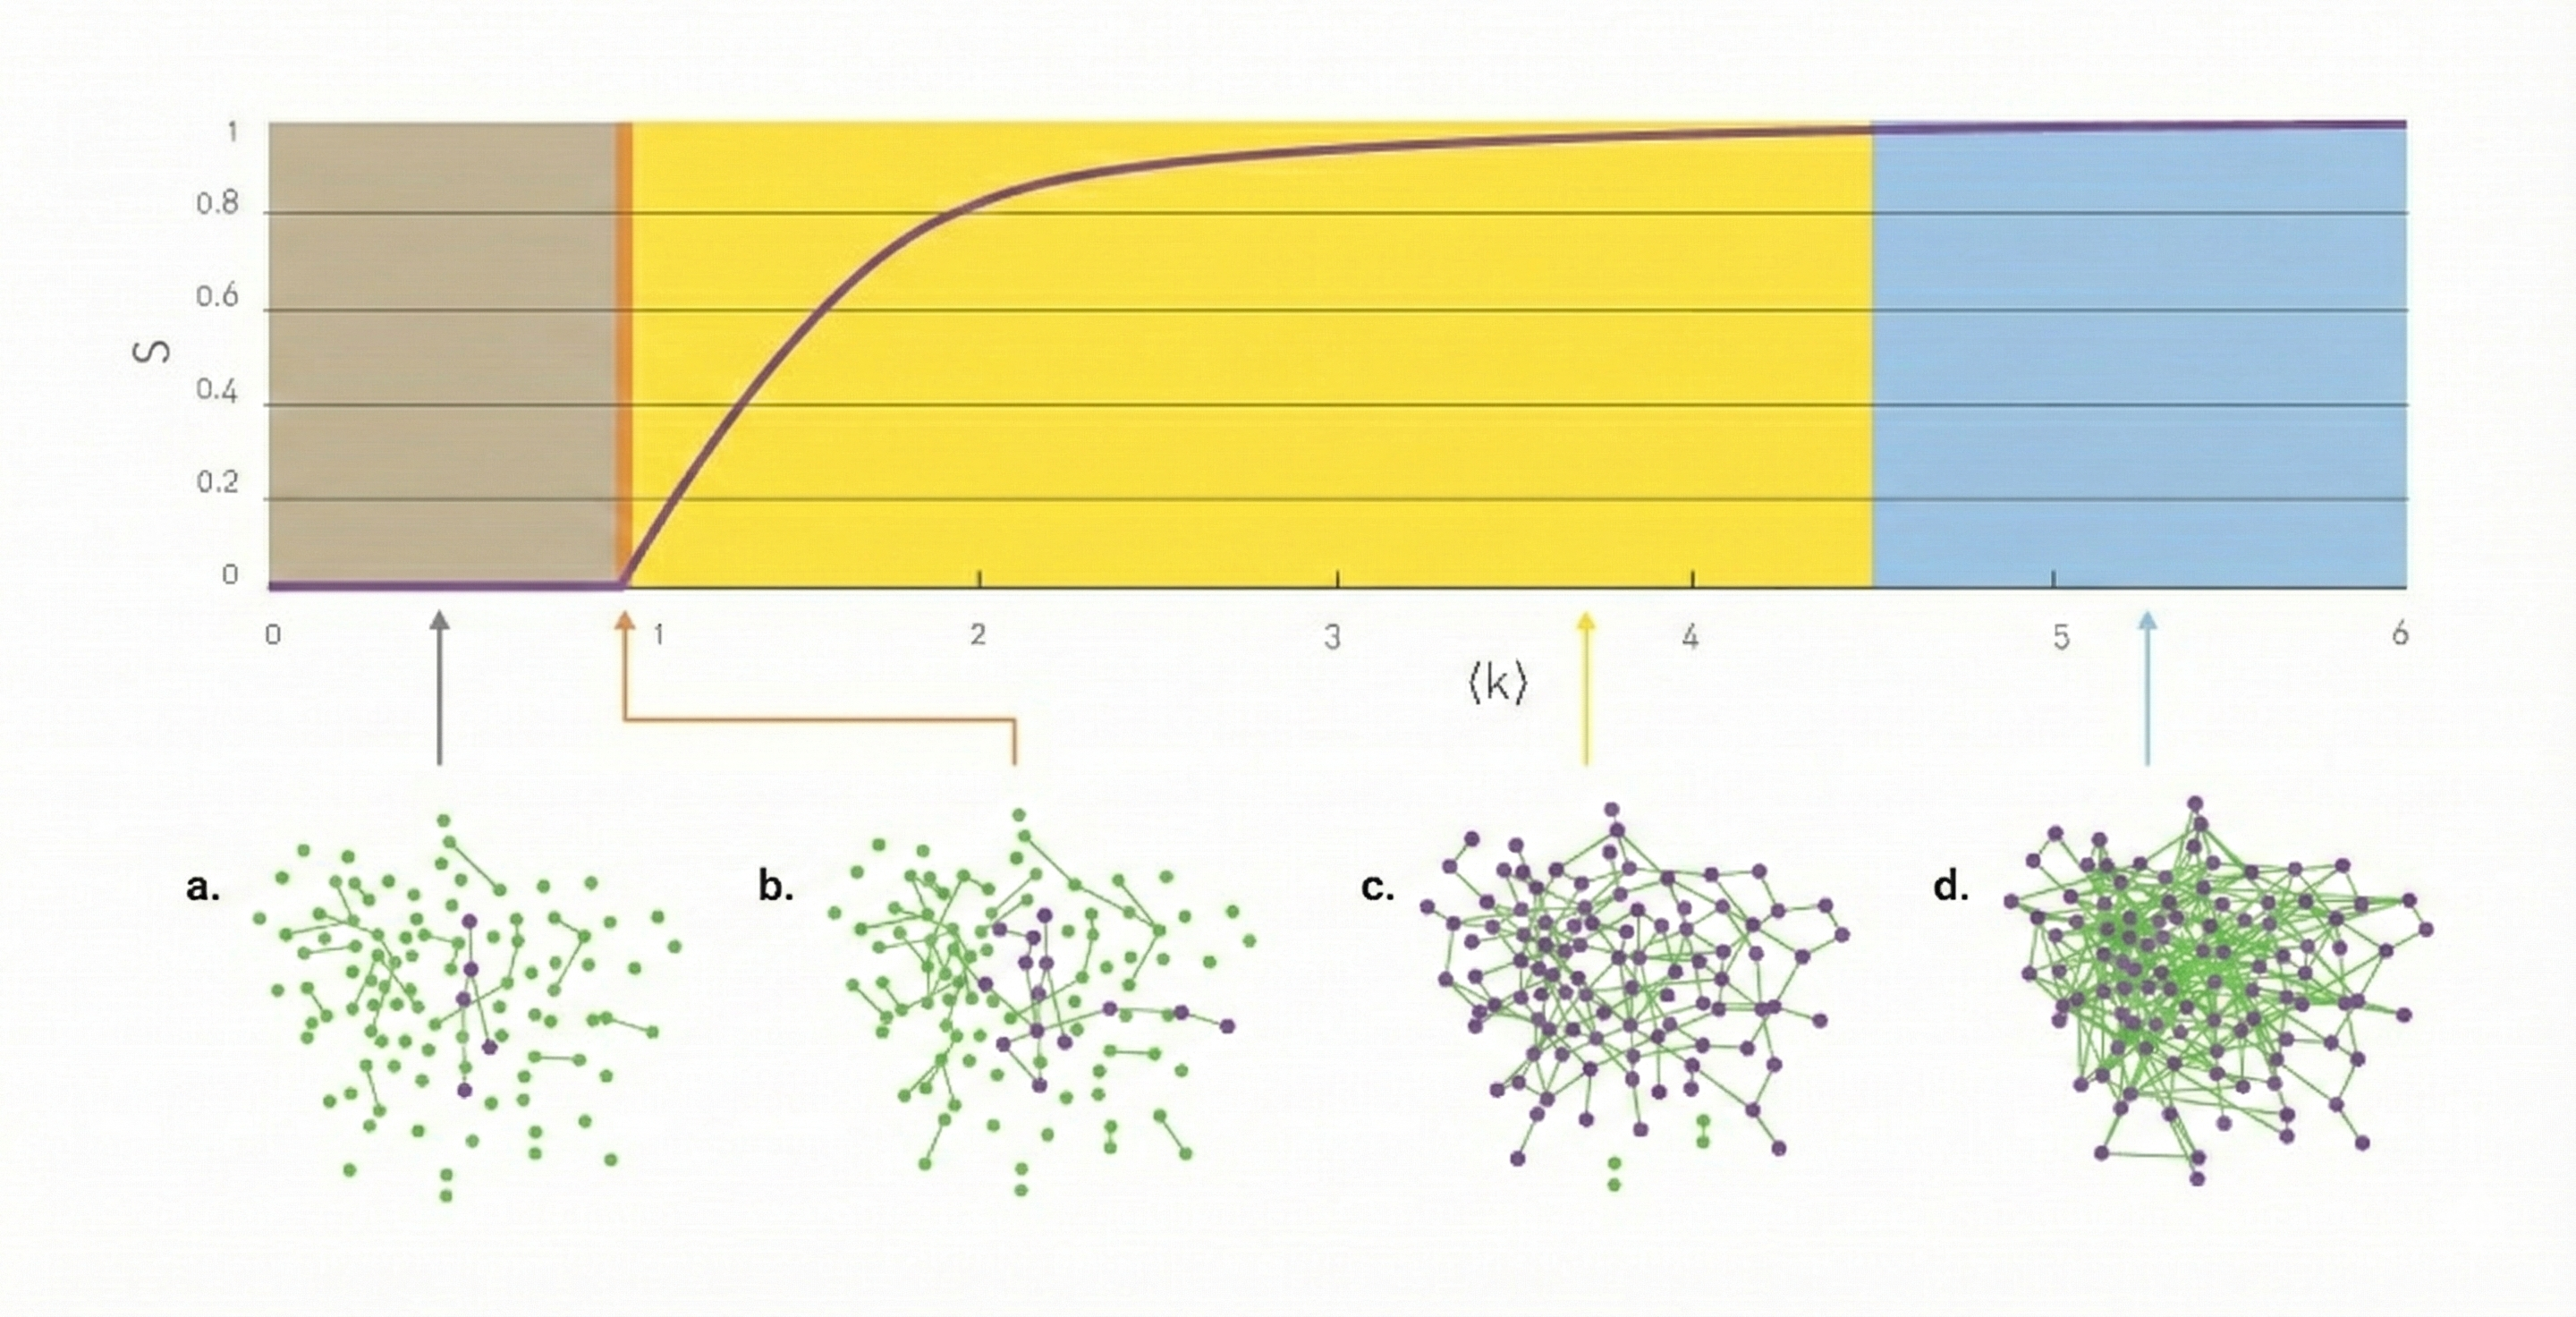
\includegraphics[width=1\textwidth]{regimes.png}
    \caption{Rappresentazione schematica dei quattro regimi topologici distinti in funzione del grado medio $\langle k \rangle$. Immagine presa da \cite[Cap. 3.6]{barabasi2016network}.}
    \label{fig:regimes}
\end{figure}

\subsection{Transizione di fase}
Per descrivere la transizione di fase possiamo introdurre due quantità fondamentali:
\begin{itemize}
    \item \textbf{Parametro d'ordine $S$:} Definito come la frazione di nodi appartenenti alla componente gigante, permette di distinguere una fase ordinata ($S > 0$) da una disordinata ($S = 0$). Per la teoria della percolazione si ha che \cite{barabasi2016network,stauffer1994introduction}:
          \begin{equation}
              S \sim (\langle k \rangle - \langle k \rangle_c)^\beta \quad\quad \langle k \rangle \to \langle k \rangle_c^+
              \label{eq:order_parameter}
          \end{equation}
          con  $\beta > 0$ esponente critico.
    \item \textbf{Suscettività $\chi$:} Definita come la dimensione media dei cluster piccoli $ \langle s \rangle$, rappresenta la sensibilità della rete a variazioni di $\langle k \rangle$. Per la teoria della percolazione si ha che \cite{barabasi2016network,stauffer1994introduction}:
          \begin{equation}    \chi \equiv \langle s \rangle \sim |\langle k \rangle - \langle k \rangle_c|^{-\gamma} \quad\quad \langle k \rangle \to \langle k \rangle_c
              \label{eq:susceptibility}
          \end{equation}
          con $\gamma > 0$ esponente critico. Ovvero la dimensione media dei cluster piccoli diverge al punto critico.
\end{itemize}

Come ricavato in \cref{sec:esponenti}, nell'intorno destro del punto critico $\langle k \rangle_c = 1$ il parametro d'ordine $S$ cresce linearmente, indicando che l'esponente critico è $\beta = 1 $. Inoltre, la suscettività $\chi$ diverge al punto critico con un esponente critico $\gamma = 1$, indicando la presenza di una transizione di fase continua (del secondo ordine) in cui la dimensione media dei cluster finiti cresce senza limiti al punto critico. Questo comportamento è analogo alla divergenza della suscettività nei sistemi termodinamici vicino al punto critico, rafforzando l'analogia tra la percolazione e le transizioni di fase in fisica statistica. Inoltre, la divergenza di $\chi$ al punto critico riflette l'emergere di cluster di tutte le dimensioni secondo una legge a potenza indicando così un'esplosione delle fluttuazioni, caratteristica universale delle transizioni di fase continue.

\section{Percolazione inversa e robustezza}
Una delle caratteristiche di maggiore interesse per un network è la sua \textbf{robustezza}, ovvero la capacità di mantenere la connettività globale nonostante la rimozione di nodi o link. La teoria della percolazione fornisce un quadro teorico per analizzare questo aspetto attraverso il concetto di \emph{percolazione inversa}, in cui si rimuovono nodi o link in modo casuale o mirato, e si studia come ciò influenzi la dimensione della componente gigante.

Analizziamo il caso della rimozione casuale di una frazione $f$ di nodi. Utilizzando il criterio di Molloy-Reed \err{REF?}:
\begin{equation}
    \frac{\langle k^2 \rangle}{\langle k \rangle} > 2
\end{equation}
il quale determina la condizione necessaria affinchè esista una componente gigante per un generico network con distribuzione dei gradi $P(k)$, è possibile derivare la soglia critica di percolazione $f_c$ \err{REF?}:
\begin{equation}
    f_c = 1 - \frac{1}{\frac{\langle k^2 \rangle}{\langle k \rangle} - 1}
\end{equation}
oltre la quale la rete collassa e perde la componente gigante. Nel caso del modello di Erdős-Rényi-Gilbert, dove $\langle k^2 \rangle = \langle k \rangle^2 + \langle k \rangle$ \err{REF?}, la soglia critica di percolazione è:
\begin{equation}
    f_c = 1 - \frac{1}{\langle k \rangle}
\end{equation}
Questo risultato mostra che la robustezza di questo network dipende unicamente dal grado medio $\langle k \rangle$: reti con grado medio più elevato sono più robuste alla rimozione casuale di nodi, poiché la soglia critica $f_c$ è più alta. Tuttavia, è sufficiente rimuovere una frazione $f_c < f < 1$ di nodi per far collassare la rete, evidenziando la vulnerabilità intrinseca del modello di Erdős-Rényi-Gilbert a fallimenti casuali.

As we
approach the percolation transition from above the network may be “functional” in
the sense of having a giant cluster, but the functional portion of the network is vanishingly small. Thus one could argue that it is misleading to interpret the percolation threshold
as the point where the network stops functioning: in effect most of it has stopped functioning
before we reach this point. To fully describe the functional state of the network one should specify
not only whether it contains a giant cluster but also what the size of that cluster is.

\ext{Questo comportamento è in contrasto con reti con distribuzioni dei gradi più eterogenee (come le reti scale-free), che possono essere molto più robuste a fallimenti casuali ma estremamente vulnerabili a attacchi mirati contro i nodi più connessi \cite[Cap. 8]{barabasi2016network}}.

\section{Simulazione e risultati}
Per verificare le previsioni teoriche, sono state condotte simulazioni numeriche in Python utilizzando la libreria \emph{igraph}.

\subsection{Transizione di fase}
Per quanto riguarda la transizione di fase, è stato creato un ensemble di $M = 20$ grafi casuali $G(N, p)$ con $N = 10^5$ nodi diversi valori di $\langle k \rangle \in [0, 5]$ . Per ogni grafo, è stata calcolata la dimensione della componente gigante $S$  (\cref{fig:S}) e la suscettività $\chi$  (\cref{fig:chi}): per ciascun valore di $\langle k \rangle$, è stato associato un valore medio di $S$ e $\chi$ calcolato sull'insieme di grafi, con incertezza data dalla deviazione standard. Per ottenere un'analisi quantitativa, si sono eseguiti fit dei dati simulati con le leggi di potenza previste dalla teoria della percolazione \eqref{eq:order_parameter} \eqref{eq:susceptibility}, al fine di estrarre gli esponenti critici $\beta$ e $\gamma$ e confrontarli con i valori teorici.

\begin{figure}[htbp]
    \centering
    \makebox[\textwidth][c]{
        \begin{minipage}{1.2\textwidth} % Allarga la riga al 120%

            \begin{subfigure}[t]{0.49\linewidth}
                \centering
                \includegraphics[width=\linewidth]{S.png}
                \caption{}
            \end{subfigure}
            \hfill
            \begin{subfigure}[t]{0.49\linewidth}
                \centering
                \includegraphics[width=\linewidth]{S_fit.png}
                \caption{.}
            \end{subfigure}

        \end{minipage}
    }
    \caption{A sinistra (a) la dimensione della componente gigante $S$ in funzione di $\langle k \rangle$. A destra (b) il fit dei dati effettuato nel range $\langle k \rangle \in [1 , 1.1]$.}
    \label{fig:S}
\end{figure}

\begin{figure}[htbp]
    \centering
    \makebox[\textwidth][c]{
        \begin{minipage}{1.2\textwidth} % Stessa larghezza per coerenza visiva

            \begin{subfigure}[t]{0.49\linewidth}
                \centering
                \includegraphics[width=\linewidth]{chi.png}
                \caption{}
            \end{subfigure}
            \hfill
            \begin{subfigure}[t]{0.49\linewidth}
                \centering
                \includegraphics[width=\linewidth]{chi_fit.png}
                \caption{}
            \end{subfigure}

        \end{minipage}
    }
    \caption{A sinistra (a) la suscettività $\chi$ in funzione di $\langle k \rangle$. A destra (b) il fit dei dati effettuato nel range $\langle k \rangle \in [0. , 0.95] \cup [1.05, 2]$.}
    \label{fig:chi}
\end{figure}

I risultati dei fit e i rispettivi valori teorici sono:
\begin{equation}
    \tilde{\chi_\beta}^2 = 4.5 \quad\quad \beta_{\text{fit}} = 0.94 \pm 0.04 \quad\quad \beta_{\text{teo}} = 1
\end{equation}
\begin{equation}
    \tilde{\chi_\gamma}^2 = 663 \quad\quad \gamma_{\text{fit}} = 0.997 \pm 0.01 \quad\quad \gamma_{\text{teo}} = 1
\end{equation}
Nonostante a livello qualitativo i dati simulati mostrino un comportamento coerente con le previsioni teoriche, a livello quantitativo si osservano deviazioni significative dagli esponenti critici teorici. Queste discrepanze potrebbero essere attribuite a diversi fattori, tra cui effetti di finite-size dovuti alla dimensione finita della rete simulata.

\subsection{Percolazione inversa}
Per quanto riguarda la percolazione inversa, è stato creato un ensemble di $M = 20$ grafi casuali $G(N, p)$ con $N = 10^5$ per diversi valori di $\langle k \rangle \in [2 , 11]$. Per ogni grafo, è stata rimossa una frazione $f$ di nodi scelti casualmente, e per diversi valori di $f \in [0,1]$ è stata calcolata la dimensione della componente gigante $S$ (normalizzata rispetto alla dimensione originale della componente gigante $S(0)$) mediando su tutti i grafi dell'ensemble, usando come incertezza la deviazione standard (\cref{fig:percolation}). Per ogni valore di $\langle k \rangle$, è stata ricavata la soglia critica di percolazione $f_c$ effettuando dei fit lineari in corrispondenza di tale punto cercando l'intercetta sull'asse x; i valori ottenuti sono poi stati riportati nel grafico (\cref{fig:fc}), nel quale si è eseguito un fit con la distribuzione teorica
\begin{equation}
    f_c = 1 - \frac{\alpha}{\langle k \rangle}
\end{equation}
dove $\alpha$ è un parametro di fit, per verificarne la coerenza con la teoria. Il risultato del fit e il rispettivo valore teorico sono:
\begin{equation}
    \tilde{\chi} = 55 \quad\quad \alpha_{\text{fit}} = 0.985 \pm 0.001 \quad\quad \alpha_{\text{teo}} = 1
\end{equation}

\begin{figure}[htbp]
    \centering
    \includegraphics[width=0.9\textwidth]{perc.png}
    \caption{Dimensione relativa della componente gigante $S(f)/S(0)$ in funzione della frazione di nodi rimossi $f$ per diversi valori di $\langle k \rangle$.}
    \label{fig:percolation}
\end{figure}

\begin{figure}[htbp]
    \centering
    \includegraphics[width=0.9\textwidth]{tresh.png}
    \caption{Soglia critica di percolazione $f_c$ in funzione di $\langle k \rangle$ con fit e funzione teorica.}
    \label{fig:fc}
\end{figure}

Anche in questo caso, nonostante a livello qualitativo i dati simulati mostrino un comportamento coerente con le previsioni teoriche, a livello quantitativo si osservano deviazioni significative dal valore teorico di $\alpha$ e un $\tilde{\chi}^2$ alto causato plausibilmente dalle basse incertezze statistiche e dalle deviazioni sistematiche di $f_c$ per $\langle k \rangle > 6$ causate da effetti di finite-size.


\section{Conclusioni}
\appendix
\section{Appendici}
\subsection{Componente Gigante}\label{sec:GC}
Sia $u$ la frazione di nodi che non appartengono alla componente gigante (GC) e $S$ la frazione di nodi che vi appartengono. Vale la relazione:
\begin{equation}
    u = 1 - S
\end{equation}
Un nodo $i$ non appartiene alla GC se, per ogni altro nodo $j$, o non esiste un arco ($1-p$) oppure esiste un arco ma $j$ non è nella GC ($pu$). La probabilità totale per un singolo nodo $j$ è
$1 - p + pu$.
Considerando tutti gli $N-1$ possibili vicini, la probabilità che $i$ non sia connesso alla GC è:
\begin{equation}
    u = (1 - p + pu)^{N-1}
\end{equation}
Sostituendo la probabilità di connessione $p = \frac{\langle k \rangle}{N-1}$, passando ai logaritmi e utilizzando l'approssimazione $\ln(1+x) \approx x$ per $x \ll 1$, otteniamo:
\begin{equation}
    \ln u = -\langle k \rangle (1-u)
\end{equation}
Esponenziando entrambi i membri otteniamo un'equazione trascendente per $u$:
\begin{equation}
    u = e^{-\langle k \rangle (1-u)}
\end{equation}
Sostituendo $u = 1 - S$, otteniamo l'equazione finale per la dimensione della GC:
\begin{equation}
    S = 1 - e^{-\langle k \rangle S}
\end{equation}
Per trovare il punto critico, cerchiamo quando la derivata del membro di destra rispetto a $S$ valutata in $S=0$ supera la pendenza della retta $y=S$ (che è 1):
\begin{equation}
    \left. \frac{d}{dS} (1 - e^{-\langle k \rangle S}) \right|_{S=0} = 1
\end{equation}
\begin{equation}
    \left. \langle k \rangle e^{-\langle k \rangle S} \right|_{S=0} = 1 \quad
\end{equation}
La transizione di fase avviene dunque a:
\begin{equation}
    \langle k \rangle_c = 1
\end{equation}

\subsection{Esponenti critici} \label{sec:esponenti}
Per quanto riguarda il parametro d'ordine, utilizzando \eqref{eq:giant_comp} possiamo espandere l'esponenziale in serie di Taylor al secondo ordine attorno a $\langle k \rangle_c = 1$ e ottenere:
\begin{equation}
    S \approx 2(\langle k \rangle - 1)
    \label{eq:S_approx}
\end{equation}
Quindi, vicino al punto critico, il parametro d'ordine cresce linearmente con $\langle k \rangle - 1$, indicando che l'esponente critico $\beta$ è pari a 1:
\begin{equation}
    S \sim (\langle k \rangle - 1)^1 \quad\quad \langle k \rangle \to 1^+
\end{equation}
Invece, per quanto riguarda la suscettività, si calcola che la dimensione media delle componenti piccole $ \langle s \rangle$, è data da \cite{newman2018networks}:
\begin{equation}
    \chi \equiv \langle s \rangle = \frac{1}{1 - \langle k \rangle + \langle k \rangle S}
    \label{eq:susceptibility_final}
\end{equation}
Nel regime subcritico ($\langle k \rangle < 1$) si ha $S = 0$, dunque:
\begin{equation}
    \chi = (1- \langle k \rangle)^{-1} \quad\quad \langle k \rangle < 1
\end{equation}
Nel regime supercritico ($\langle k \rangle > 1$), sostituendo \eqref{eq:S_approx} in \eqref{eq:susceptibility_final}, si ottiene:
\begin{equation}
    \chi = \frac{1}{1 - \langle k \rangle + 2(\langle k^2 \rangle - \langle k \rangle)} \quad\quad  \langle k \rangle \to 1^+
\end{equation}
scrivendo $\langle k \rangle = 1 + \epsilon$ con $\epsilon \to 0^+$, tenendo solo il termine lineare in $\epsilon$, si ottiene:
\begin{equation}
    \chi \approx \frac{1}{- \epsilon + 2\epsilon} = \frac{1}{\epsilon} = ( \langle k \rangle - 1)^{-1} \quad\quad  \langle k \rangle \to 1^+
\end{equation}
quindi la suscettività diverge al punto critico con un un esponente critico $\gamma = 1$:
\begin{equation}
    \chi \sim |\langle k \rangle - 1|^{-1} \quad\quad \langle k \rangle \to 1
\end{equation}


\printbibliography[heading=bibintoc, title={Bibliografia}]

\end{document}